\chapter {Listo de la primitivoj}
\label{liste-prim} 

Kiel dirite anta^ue, oni kontrolas la testudon per internaj komandoj
nomataj prakomandoj a^u \og primitivoj\fg.  Jen klasado de tiuj
primitivoj:

\section{Movi la testudon, administri la krajonon kaj la kolorojn}
\subsection{Movi}
Primitivoj por movi la testudon.

\prim{anta^uen, an, antauen, antawen, antauxen} {n}
Movas la testudon anta^uen je $n$ pa^soj la^u la nuna direkto.

\prim{malanta^uen, man, malantauen, malantawen, malantauxen}{n}
Movas la testudon malanta^uen je $n$ pa^soj la^u la nuna direkto.

\prim{dekstren, dn}{n}
Turnas la testudon je $n$ gradoj dekstren rilate al la nuna direkto.

\prim{maldekstren, mdn}{n}
Turnas la testudon je $n$ gradoj maldekstren rilate al la nuna direkto.

\prim{rondon\_desegnu, rond}{R}
Desegnas cirklon kun radiuso R ^cirka^u la testudo.

\prim{arkon\_desegnu, ark}{R angulo1 angulo2}
Grafiki cirklan arkon kun radiuso R ^cirka^u la testudo, de la angulo 
1 ^gis la angulo 2.  (Angulo 0 estas alsupre kaj 
kreskas horlo^ge.)

\prim{originen, o}{}
Remetas la testudon en ^gian komencan situon, tio estas, en la punkton
kun koordinatoj {[}0 0{]} kaj rigardanta supren.

\prim{situon\_provizu, sitp}{listo}
Movas la testudon en punkton kun koordinatoj indikitaj de la listo de 
du nombroj (absciso kaj ordinato).

\prim{x\_provizu, xp}{x}
Movas horizontale la testudon ^gis la punkto kun absciso x.

\prim{y\_provizu, yp}{y}
Movas vertikale la testudon ^gis la punkto kun ordinato x.

\prim{xy\_provizu,xyp}{x y}
 Same kiel sitp{[}x y{]}

\prim{direkton\_provizu, dirp}{n}
Direktas la testudon al la angulo indikita.  $0$ signifas vertikale 
alsupre; turni kiel indikiloj de horlo^go.

\prim{etikedu, etik}{vortolisto}
Desegnas la vorton a^u la liston indikitan, tie kie trovi^gas 
la testudo kaj la^u ^gia inklino.
Ekzemple: \texttt{etikedu [Saluton al vi]} skribos la frazon 
\og Saluton al vi\fg{} tie kie estas lokita la testudo
kaj respektante la direkton de ^gi.

\prim{punkton\_montru, punkt}{listo}
^Saltas la punkton difinitan de la koordinatoj de la listo (je la 
koloro de krajon').

\subsection{Atributoj de la testudo}

La primitivoj prezentotaj ^ci tie ebligas modifi l' atributojn de la
testudo.  Por ekzemplo, ^cu necesas ke la testudo estu videbla sur l'
ekrano?  Je kiu koloro ^gi skribu kiam ^gi movi^gos?

\prim{testudon\_montru, tdm}{}
Videbligu la testudon sur l' ekrano.

\prim{testudon\_ka^su, tdk}{}
Malvidebligu la testudon sur l' ekrano.

\prim{ekranon\_vi^su, ev}{}
Forvi^su la desegnejon kaj remetu la testudon en ^gian komencan situon.

\prim{purigu, pur}{}
Forvi^su la desegnejon sed lasu la testudon sur la sama loko.

\prim{pradifine, pradif}{}
Forvi^su la desegnareon kaj valorigu la^u la apriorajn valorojn kelkajn 
parametrojn:
\begin{itemize}
 \item krajonkoloro: nigra
 \item ekrankoloro: blanka
 \item moduso movada: mal^saltita
 \item tiparo por la grafikejo kaj la historiejo: Dialog 12 punktoj
 \item krajonformo: kvadrata
 \item desegna kvalito: normala
 \item maksimuma nombro de testudoj: 16
 \item moduso kontrolo: mal^saltita
 \item ekranamplekso: 1000x1000
\end{itemize}

\prim{mallevu, ml}{}
La testudo skribu kiam ^gi movi^gas.

\prim{levu, l}{}
La testudo ne skribu plu kiam ^gi movi^gas.

\prim{gumskrapu, gum}{}
La testudo forvi^sas ^ciun skriba^jon trovitan.

\prim{strekon\_inversu, si}{}
Mallevu la krajonon kaj metu la testudon en moduson inversi.

\prim{desegne, dsg}{}
Mallevu la krajonon kaj metu ^gin en moduson de klasika desegno.

\prim{skribkoloron\_provizu, skolp}{entjer-listo [r v b]}
\label{fcc} Establu la koloron de la krajono.  Rigardu p.~\pageref{couleurs}.

\prim{fonkoloron\_provizu, fkolp}{entjer-listo [r v b]}
\label{fcfg}  
Establu la koloron de la ekranfono.  Rigardu p.~\pageref{couleurs}.

\prim{situon, sit}{}
Redonu la nunan situon de la testudo.  Ekz.: \texttt{sit} redonus
{[}10 -100{]}

\prim{direkton, dir}{}
Redonas la direkton de la testudo (rigardu \texttt{fixecap}).

\prim{aldirektu, diral}{listo}
La listo enhavu du nombrojn prezentantajn koordinatojn.  ^Gi redonas 
la direkton kiu necesas doni al la testudo
por iri ale al la punkto difinita de la koordinatoj de la listo.

\prim{distancon, dist}{listo}
La listo enhavu du nombrojn prezentantajn koordinatojn.  
^Gi redonas la nombron de pa^soj inter la nuna situ kaj
la punkto difinita de la koordinatoj de la listo.

\prim{skribkoloron, sk}{}
Redonu la nunan koloron de la krajono.  Tiu koloro estas indikita 
per listo [r v b] kie r estas la konsista^jo 
ru^ga, b la blua kaj v la verda.

\prim{fonkoloron, fkol}{}
Redonu la nunan koloron de la ekranfono.  Tiu koloro estas indikita 
per listo [r v b].

\prim{volve, vlv}{}
Agordu la ekranliman moduson, tiel ke se la testudo eliras
el la desegnejo, ^gi reaperas sur la mala flanko!

\prim{fenestre, fen}{}
Agordu la ekranliman moduson, tiel ke la testudo estas libera 
por eliri en la desegnejo.
Kompreneble, ^gi ne skribas ekster la desegnejo.

\prim{ferme, f}{}
Agordu la ekranliman moduson, tiel ke la testudo restu en la desegnejo.  
Se ^gi devus eliri, erarmesa^go avertos kaj donos la maksimuman 
pa^snombron anta^u ol eliri.

\prim{perspektive}{}
Agordu la desegnejon, tiel ke la testudo povu direkti^gi en la spaco.
(Rigardu la sekcion \ref{3D} dedi^cita al tiu moduso.)
Por eliri el tiu moduso, uzu la primitivon \texttt{fenestre}, 
\texttt{volve} a^u \texttt{ferme}.

\prim{koloron, kol}{listo}
Redonu la koloron de la pikselo (rastrumero) kun koordinatoj de la listo.
Tiu koloro prezenti^gas kiel listo [r v b].

\prim{skribdikon\_provizu, sdikp}{nombro}
Establu la dikecon de la krajonpinto la^u pikseloj.
Apriore ^gi valoras $1$.

\prim{skribdikon, sdik}{}
Redonu la dikecon de la krajonpinto la^u pikseloj. 

\prim{sformp, skribformon\_provizu}{0-1}
Establu la formon de la krajonpinto.
\begin{itemize}
\item 0$\to$kvadrata.
\item 1$\to$ronda.
\end{itemize}
\noindent

\prim{sform, skribformon}{}
Redonu la formon de la krajonpinto. 0$\to$kvadrata. 1$\to$ronda.

\prim{dsgcp, desegnecon\_provizu}{0-1-2}
Establu desegnan kvaliton.
\begin{itemize}
 \item 0$\to$normala.
 \item 1$\to$alta.
 \item 2$\to$malalta.
\end{itemize}
\noindent

\prim{dsgc, desegnecon}{}
Redonas la kvaliton de desegnado.
\begin{itemize}
 \item 0$\to$normala.
 \item 1$\to$alta.
 \item 2$\to$malalta.
\end{itemize}
\noindent

\prim{dsgamplp, desegnamplekson\_provizu}{listo}
Establu l' amplekson de la desegnejo.

\prim{dsgampl, desegnamplekson}{}
Redonu la amplekson de la desegnejo.

\prim{formon\_provizu, formp}{entjero}
Vi povas elekti l' aspekton de la testudo uzata, ^cu per Elekto - 
Preferoj - Elektu testudon, ^cu per tiu primitivo.  La nombro devas
esti entjero inter $0$ kaj $6$ ($0$ indikas la trilateran formon).

\prim{formon, form}{}
Redonas numeron kiu reprezentas la nunan bildon de la testudo.

\prim{tiparon\_provizu, tipp}{entjero}
Kiam oni skribas tekston sur l' ekrano per la primitivo \texttt{etikedu},
eblas modifi la amplekson de la tiparo uzata, per tiu primitivo.
Apriore, l' amplekso estas $12$.

\prim{tiparon, tip}{}
Redonas la amplekson de la tiparo nun uzata kiam oni skribas per la 
primitivo \texttt{etiquette}.

\prim{tiparnomon\_provizu, tipnp}{entjero}
Establu la tiparon uzata por skribi sur l' ekrano per la primitivo 
\texttt{etikedu}.  La numero indikanta la tiparon uzotan estas trovebla
en Menuo - Elektoj - Preferoj - Langeto Tiparo.

\prim{tiparnomon, tipn}{}
Redonu liston konsistanta el du eroj.  La unua estal la numero de la
tiparo uzata por skribi per la primitivo \texttt{etikedu}. 
La dua estas listo enhavanta la nomon de tiu sama tiparo.

\prim{ekranon\_disigu}{nombro}
Establu la proporcio inter la grafikejo kaj la historiejo.
La nombro estu inter $0$ kaj $1$.  Kiam ^gi valoras $1$
la desegnejo okupas ^ciom; kiam $0$, la historiejo okupas ^ciom.

\prim{ekranon\_disigon}{}
Redonas la proporcion nunan inter la desegnejo kaj la historiejo.

\prim{dratretu}{a b}
a kaj b estas entjeroj.  ^Gi desegnas dratreton kies ^ciu ^celo
grandas a mul b.

\prim{neplu\_dratretu}{}
Forigas la dratreton.

\prim{dratretkoloron\_provizu}{koloro}
Ebligas elekti la koloron de la dratreto.
Ekzemple: \texttt{dratretkoloron\_provizu ru^gan}

\prim{dratreta\_koloron}{}
Redonas la nunan koloron de la dratreto.

\prim{dratreta?}{}
Testu ^cu la dratreto desegnitas, kaj redonu \emph{vera} a^u \emph{malvera} 
la^u la okazo.

\prim{aksigu}{n}
Grafiku la du aksojn.  La indikiloj estas disigitaj de $n$ testudpa^soj.

\prim{x\_aksigu}{n}
Grafiku la horizontalan akson.  L' indikilojn disigas $n$ testudpa^soj.

\prim{y\_aksigu}{n}
Grafiku l' vetikalan akson.  L' indikilojn disigas $n$ testudpa^soj.

\prim{aksojn\_vi^su}{}
Forigu la aksojn.\\

\prim{akskoloron\_provizu}{koloro}
Establu la koloron de la aksoj. Ekzemple: \texttt{akskoloron\_provizu
  [120 5 100]} \\

\prim{akskoloron}{}
Redonas la nunan koloron de la aksoj.

\prim{x\_aksa?}{}
Testu ^cu la horizontala akso estas grafikita.  Redonu \emph{vera}
a^u \emph{malvera} la^u l' okazo.

\prim{y\_aksa?}{}
Testu ^cu la vertikala akso estas grafikita.  Redonu \emph{vera}
a^u \emph{malvera} la^u l' okazo.

\prim{zomu}{n}
Zomu al la desegnejo.  La argumento \texttt{n} reprezentas
la skalon rilate al l' amplekso de la bildo establita en la
preferejo.

\prim{fenestramplekson, fenampl}{}
Redonu liston formita de la koordinatoj de la angulo supra maldekstra
de la desegnejo kaj de la angulo malsupra dekstra.

\prim{avertu, avrt}{listo}
Skribu informa mesa^gon en dialogfenestron; programrulado haltas ^gis
jesa musklako.

\prim{etikedlongon, etikl}{vortolisto}
Redonu la longon necesan por skribi la vorton a^u la liston sur la
desegnareon uzante la elektitan tiparon.  Tiun longon oni esprimu per
testudpa^soj.

\subsection{Iom pri l' koloroj}

En XLogo la kolorojn oni difinas per tri nombroj inter $0$ kaj $255$.
Tiu koda sistemo nomi^gas \og RVB\fg{} (ru^ga, verda, blua).  ^Ciu
nombro respondas al la respektiva intenseco de la ru^go, la verdo kaj
la bluo por la konsiderata koloro.  ^Car tio ne estas tre intuicia,
XLogo proponas anka^u $16$ anta^udifinitaj koloroj uzeblaj ^cu per
numero, ^cu per primitivo. \label{couleurs}

\begin{center}
  \begin{longtable}{*{4}{|c}|} \hline
    Numero & Primitivoj & [R V B] & Koloro \\ 
    \hline
    0& \texttt{nigra} & [0 0 0] & \index{noir}
    \begin{minipage}[m]{1.5cm}
      \begin{center}
        \vspace{0.2cm}
        
\includegraphics[width=1 cm]{bildoj/couleur0.png}
        \vspace{0.2cm}
      \end{center}
    \end{minipage}\\
    \hline
    1 & \texttt{ru^gan} & [255 0 0] & \index{rouge}
    \begin{minipage}[m]{1.5cm}
      \begin{center}
        \vspace{0.2cm}
        
\includegraphics[width=1 cm]{bildoj/couleur1.png}
        \vspace{0.2cm}
      \end{center}
    \end{minipage}\\\hline
    2 & \texttt{verdan} & [0 255 0] & \index{vert}
    \begin{minipage}[m]{1.5cm}
      \begin{center}
        \vspace{0.2cm}
        
\includegraphics[width=1 cm]{bildoj/couleur2.png}
        \vspace{0.2cm}
      \end{center}
    \end{minipage}\\
    \hline
    3 & \texttt{flavan} & [255 255 0] & \index{jaune}
    \begin{minipage}[m]{1.5cm}
      \begin{center}
        \vspace{0.2cm}
        
\includegraphics[width=1 cm]{bildoj/couleur3.png}
        \vspace{0.2cm}
      \end{center}
    \end{minipage}\\
    \hline
    4 & \texttt{bluan} & [0 0 255] & \index{bleu}
    \begin{minipage}[m]{1.5cm}
      \begin{center}
        \vspace{0.2cm}
        
\includegraphics[width=1 cm]{bildoj/couleur4.png}
        \vspace{0.2cm}
      \end{center}
    \end{minipage}\\
    \hline
    5 & \texttt{violru^gan} & [255 0 255] & \index{magenta}
    \begin{minipage}[m]{1.5cm}
      \begin{center}
        \vspace{0.2cm}
        
\includegraphics[width=1 cm]{bildoj/couleur5.png}
        \vspace{0.2cm}
      \end{center}
    \end{minipage}\\
    \hline
    6 & \texttt{verdbluan} & [0 255 255] & \index{cyan}
    \begin{minipage}[m]{1.5cm}
      \begin{center}
        \vspace{0.2cm}
        
\includegraphics[width=1 cm]{bildoj/couleur6.png}
        \vspace{0.2cm}
      \end{center}
    \end{minipage}\\
    \hline
    7 & \texttt{blankan} & [255 255 255] & \index{blanc}
    \begin{minipage}[m]{1.5cm}
      \begin{center}
        \vspace{0.2cm}
        
\includegraphics[width=1 cm]{bildoj/couleur7.png}
        \vspace{0.2cm}
      \end{center}
    \end{minipage}\\
    \hline
    8 & \texttt{grizan} & [128 128 128] & \index{gris}
    \begin{minipage}[m]{1.5cm}
      \begin{center}
        \vspace{0.2cm}
        
\includegraphics[width=1 cm]{bildoj/couleur8.png}
        \vspace{0.2cm}
      \end{center}
    \end{minipage}\\
    \hline
    9 & \texttt{hele\_grizan} & [192 192 192] & \index{grisclair}
    \begin{minipage}[m]{1.5cm}
      \begin{center}
        \vspace{0.2cm}
        
\includegraphics[width=1 cm]{bildoj/couleur9.png}
        \vspace{0.2cm}
      \end{center}
    \end{minipage}\\
    \hline
    10 & \texttt{malhele\_ru^gan} & [128 0 0] & \index{rougefonce}
    \begin{minipage}[m]{1.5cm}
      \begin{center}
        \vspace{0.2cm}
        
\includegraphics[width=1 cm]{bildoj/couleur10.png} 
        \vspace{0.2cm}
      \end{center}
    \end{minipage}\\
    \hline
    11 & \texttt{malhele\_verdan} & [0 128 0] & \index{vertfonce}
    \begin{minipage}[m]{1.5cm}
      \begin{center}
        \vspace{0.2cm}
        
\includegraphics[width=1 cm]{bildoj/couleur11.png}
        \vspace{0.2cm}
      \end{center}
    \end{minipage}\\
    \hline
    12 & \texttt{malhele\_bluan} & [0 0 128] & \index{bleufonce}
    \begin{minipage}[m]{1.5cm}
      \begin{center}
        \vspace{0.2cm}
        
\includegraphics[width=1 cm]{bildoj/couleur12.png}
        \vspace{0.2cm}
      \end{center}
    \end{minipage}\\
    \hline
    13 & \texttt{oran^gkoloran} & [255 128 0]& \index{orange}
    \begin{minipage}[m]{1.5cm}
      \begin{center}
        \vspace{0.2cm}
        
\includegraphics[width=1 cm]{bildoj/couleur13.png}
        \vspace{0.2cm}
      \end{center}
    \end{minipage}\\
    \hline
    14 & \texttt{rozan} & [255 175 175] & \index{rose}
    \begin{minipage}[m]{1.5cm}
      \begin{center}
        \vspace{0.2cm}
        
\includegraphics[width=1 cm]{bildoj/couleur14.png}
        \vspace{0.2cm}
      \end{center}
    \end{minipage}\\
    \hline
    15 & \texttt{violan} & [128 0 255] & \index{violet}
    \begin{minipage}[m]{1.5cm}
      \begin{center}
        \vspace{0.2cm}
        
\includegraphics[width=1 cm]{bildoj/couleur15.png}
        \vspace{0.2cm}
      \end{center}
    \end{minipage}\\
    \hline
    16 & \texttt{maronan} & [153 102 0] & \index{marron}
    \begin{minipage}[m]{1.5cm}
      \begin{center}
        \vspace{0.2cm}
        
\includegraphics[width=1 cm]{bildoj/couleur16.png}
        \vspace{0.2cm}
      \end{center}
    \end{minipage}\\
    \hline
  \end{longtable} 
\end{center}

\begin{verbatim}
# Jenaj tri komandoj efikas same
skolp oranĝkoloran
skolp 13
skolp [255 200 0]
\end{verbatim}

\subsection{La moduson movado (animado)}

Ekzistas tri primitivoj: \texttt{movado}, \texttt{neplu\_movigu}
kaj \texttt{novigu}; kiuj ebligas ruli komandojn sen ke la testudo
montru la rezultojn.

\prim{movado}{}

^Saltu moduson movado.  La testudo ne plu desegnu sur l' ekrano, sed
nur en memoro.  Por ^gisdatigi la desegnon sur l' ekrano, uzu la 
primitivon \texttt{rafraichis}.  Tre utila por krei animadon a^u por
desegni pli rapide.

\prim{neplu\_movigu}{}

Tio haltigas la moduson movado: oni revenas en moduson klasikan, do
oni tuj vidas la movojn de la testudo sur l' ekrano.

\prim{novigu}{}

En moduso movado, novigu l' ekranon: la bildo sur la desegnejo estu
^gisdatigita.

Por indiki la moduson movado, ikono prezentanta fotilon aperas en la
historiejo.  Se vi klakos la fotilon, l' animado haltos; do tio egalas
uzi la primitivon \texttt{neplu\_movigu}.
\begin{center}
   
\includegraphics[scale=2.5]{bildoj/animation.png}
\end{center}

\subsection{Skribi tekston en la historiejo}

Tiu tabelo grupas la primitivojn rilatajn al la historiejo.
^Ciu primitivo rilata al la amplekso kaj la koloro de la tiparo uzata,
nur validas por la rezulto de la primitivo \texttt{skribu}.

\prim{tv, tekston\_vi^su}{}

Purigas la areon enhavantan la historion de la komandoj kaj komentarioj.

\prim{s, skribu}{arg1}

Skribu l' argumenton \textit{arg1} en la historiejon.

\begin{verbatim}
skribu "abcd --------> abcd
s [1 2 3 4] ----> 1 2 3 4
s 4 ------------> 4
\end{verbatim}

\prim{tajpu}{arg1}

Same kiel la primitivo \texttt{skribu} sed ^gi ne saltas linion.

\prim{teksttiparon\_provizu, ttipp}{n}

Difinu l' amplekson de la tiparo en la historiejo.  Valida nur por la
primitivo \texttt{skribu}.

\prim{teksttiparon, ttip}{}

Redonas la amplekson de la tiparo uzata de la primitivo \texttt{skribu}.

\prim{tekstkoloron\_provizu, tkolp}{koloro}

Difinu la koloron de la tiparo en la historiejo.  Valida nur por la 
primitivo \texttt{skribu}.  Rigardu p.~\pageref{couleurs}.

\prim{tekstkoloron, tkol}{}

Redonas la koloron de la tiparo uzata de la primitivo \texttt{skribu}
en la historiejo.

\prim{teksttiparnomon\_provizu, ttipnp}{n}

Establu la tiparon uzatan por skribi en la historiejo per la primitivo
\texttt{skribu}.  La numero de la tiparo estas ser^cebla en 
Menuo$\to$Elektu$\to$Preferoj$\to$Langeto Tiparo.

\prim{teksttiparnomon, ttipn}{}

Redonas liston konsistanta el du eroj.  La unua estas la numero
reprezentanta la tiparon uzatan por skribi sur l' ekrano per la
primitivo \texttt{skribu}.  La dua estas listo enhavanta la nomon de
tiu sama tiparo.

\prim{stilon\_provizu, stip}{arg1}

Establu la stilon de la tiparo uzata de la primitivo
\texttt{skribu}.  La stiloj elekteblaj estas \texttt{simple,
  dike, kursive, forstreke, indice, eksponente, substreke}. 
Se vi deziros uzi plurajn samtempe, indiku ilin en listo.

Jen kelkaj ekzemploj por formati la tekston per la primitivo \texttt{skribu}:\\ \\
\texttt{stilon\_provizu [dike substreke] skribu "saluton}\\
\textbf{\underline{bonjour}}\\
\texttt{stip "forstreke tajpu [teksto forstrekita] stip "kursive tajpu "\textbackslash\ x stip "eksponente skribu 2}\\
\sout{teksto forstrekita} $x^2$

\prim{sti, stilon}{}

Redonu liston konsistantan el la malsamaj setiloj nun uzataj de la
primitivo \texttt{skribu}.

\section{La testudo en la spaco} \label{3D}

De la versio 0.9.92, la testudo povas eliri el la ebeno por movi^gi
en la spaco.  Por tio oni uzu la primitivon \texttt{perspektive}.
Bonvenon en la mondon de la 3D-perspektivo!

\subsection{La perspektiva te^hniko}

Por prezenti la spacon tridimensian en ebeno nur dudimensia, oni uzu
projektan perspektivon.  Kamerao rigardas la 3D-scenon kaj ^gia vidado estas projektata sur intermezan ebenon.
Jen skemo ilustranta tiun te^hnikon.

\begin{center}
\includegraphics*[scale=0.6]{bildoj/perspective.png}
\end{center}

Kelkaj primitivoj ebligas loki la kameraon la^u via volo, kun la
projekta ekrano ^guste je duona distanco.

\subsection{Kompreni la movojn en la spaco}

Sur la ebeno, testudan direkton difinas nur l' angulo rilate al la
vertikalo.  En la spaco, la direkton donas $3$ angulaj valoroj:

\begin{itemize}
\item La flankklino: La testuda klino la^u la akso $(Oy)$
\item La frontklino: La^u la akso $(Ox)$
\item Le direkto: La^u l' akso $(Oz)$ 
\end{itemize}

Efektive, por movi^gi en la spaco, la testudo kondutas kiel aviadilo.
Jen malgranda skemo ebliganta prezenti tiujn magnitudojn:

\begin{minipage}{5.8cm}
\begin{center}
\includegraphics*[scale=0.3]{bildoj/plane-roll.png}
\textbf{La flankklino}
\end{center}
\end{minipage}
\begin{minipage}{5.5cm}
\begin{center}
\includegraphics*[scale=0.35]{bildoj/plane-pitch.png}
\textbf{La frontklino}
\end{center}
\end{minipage}
\begin{minipage}{5.5cm}
\begin{center}
\includegraphics*[scale=0.3]{bildoj/plane-heading.png}
\textbf{La direkto}
\end{center}
\end{minipage}

Tio povas ^sajni komplikita komence, sed rimarku ke multaj aferoj 
rilatas al kutimaj movoj sur l' ebeno.

\prim{an, anta^uen, man, malanta^uen}{n}

Sama konduto kiel sur l' ebeno.

\prim{dn, dekstren, mdn, maldekstren}{n}

Same kondutas kiel sur l' ebeno.

\prim{dfn, dekstraflanken}{n}

La testudo pivotas dekstren la^u ^gia longeca akso je $n$ gradoj.

\prim{mdfn, maldekstraflanken}{n}

La testudo pivotas madekstren la^u ^gia longeca akso je $n$ gradoj.

\prim{supren}{n}

La testudo pivotas supren la^u ^gia lar^geca akso je $n$ gradoj.

\prim{malsupren}{n}

La testudo pivotas supren la^u ^gia lar^geca akso je $n$ gradoj.

Sur l' ebeno por grafiki kvadraton je latero $200$:
\begin{verbatim}
 ripetu 4 [an 200 dn 90] 
\end{verbatim}

Tiuj komandoj restas validaj en la spaco, kaj la kvadrato estas desegnita perspektive.
Se oni turnus \og malsupren\fg\ la testudon je $90$ gradoj oni povus grafiki tiam novan kvadraton.

\begin{minipage}{7cm}
\begin{verbatim}
ev
ripetu 4 [an 200 dn 90]
malsupren 90
ripetu 4 [an 200 dn 90]
\end{verbatim}
\end{minipage}
\begin{minipage}{10cm}
  \begin{center}
    \includegraphics*[scale=0.4]{bildoj/perspective1.png}
  \end{center}
\end{minipage}

Restas trejni sin por lerni ^ciun eblan direkton!

Necesas ^ciuokaze kompreni ke la tri turnaj primitivoj estas reciproke ligitaj.
Por ekzemplo, provu la jenan sinsekvon:

\begin{minipage}{7cm}
\begin{verbatim}
ev
mdfn 90 supren 90 dfn 90
\end{verbatim}
\end{minipage}
\hspace{3cm}
\begin{minipage}{7cm}
  \begin{center}
    La movo farita estus egala al fari \texttt{maldekstren 90} 
    (provu simuli la testudon per via mano, ekzemple...).
  \end{center}
\end{minipage}

\subsection{Listo de aliaj primitivoj}

^Ciuj sekvaj primitivoj valoras en la spaco kaj sur l' ebeno.  La sola
diferenco estas la naturo de la argumentoj atendataj a^u la naturo de
la respondoj.  Por ekzemplo, la primitivo \texttt{sitp} ou
\texttt{situon\_provizu} atendas ^ciam liston kiel argumenton, sed nun
necesas ke tiu listo enhavu tri nombrojn $(x;y;z)$ reprezentantajn la
spacajn koordinatojn de la dezirata punkto.  Jen resumo de tiuj
komandoj:

\subsubsection{Primitivoj validaj kaj sur l' ebeno kaj en la spaco}

\begin{center}
  \begin{tabular}{|cccc|}
    \hline
    \texttt{rond, rondon\_desegnu}&
    \texttt{ark, arkon\_provizu}&
    \texttt{o, originen}&
    \texttt{diral, aldirektu}\\
    \hline
    \texttt{dist, distancon}&
    \texttt{sitp, situon\_provizu}&
    \texttt{xp, x\_provizu}&
    \texttt{yp, y\_provizu}\\
    \hline
    \texttt{dirp, direkton\_provizu}&
    \texttt{etikedu}&
    \texttt{etikedlongon, etikl}&
    \texttt{punkt, punkton\_montru}\\
    \hline
    \texttt{sit, situon}&
    \texttt{dir, direkton} & &\\
    \hline
  \end{tabular} 
\end{center}

\subsubsection{Primitivoj validaj nur en moduso 3D}

\prim{xyzp, xyz\_provizu}{x y z}

Tiu primitivo movas la testudon al la punkto kun koordinatoj
indikitaj.  ^Gi atendas tri argumentojn; tiu primitivo similas al
\texttt{sitp} krom ke la koordinatojn oni ne indikas en listo. 

Ekzemplo, \texttt{xyzp -100 200 50}: movu la testudon al punkto je
koordinatoj $x=-100;y=200;z=50$.

\prim{zp, z\_provizu}{z}

Tiu primitivo movas la testudon al punkto kies koordinato $z$ egalas
l' argumenton indikitan.  ^Gi atendas do nombron kiel argumenton; tiu
primitivo estas komparebla al \texttt{xp} kaj \texttt{yp}.

\prim{orientadon\_provizu}{listo}

Loku la testudon la^u la dezirata klino.  Tiu primitivo atendas liston
enhavantan tri nombrojn, respektive la flankklinon, la frontklinon kaj
la direkton.

Ekzemple, \texttt{orientadon\_provizu [100 0 58]}: la testudo i^gos
flankklina je $100$ gradoj, frontklina je $0$ gradoj kaj direkta je
$58$ gradoj.

\prim{orientadon}{}

Redonas l' orientadon de la testudo kiel liston enhavantan respektive
la flankklinon, la frontklinon kaj la direkton.  Atentu l' ordon de
tiuj nombroj; ekzemple, se l' orientado estas \texttt{[100 20 90]},
tio signifas ke por atingi la saman orientadon, de la komenca situo
(ekzemple post vi^si l' ekranon), necesos tajpi:

\begin{center}
  \texttt{dekstraflanken 100 supren 20 dekstren 90}
\end{center}

Se vi permutus l' ordon de tiuj instrukcioj, vi ne akirus l'
orientadon deziratan!

\prim{flankklinon\_provizu}{n}

Pivotigu la testudon la^u ^gia longeca akso tiel ke ^gi prenu l'
frankklinon indikitan.

\prim{flankklinon}{} 

Redonas la nunan valoron de la flankklina angula.

\prim{frontklinon\_provizu}{n} 

Pivotigu la testudon la^u ^gian lar^geca akso tiel ke ^gi prenu la
frontklinan angulon indikitan.

\prim{frontklinon}{} 

Redonas la nunan valoron de la frontklinan angulon.

\subsection{La 3D-modelilo}

\xlogo{} havas modelilon 3D kiu ebligas montri vian tridimensian
grafika^jon en sceno kun lumoj kaj mallumoj.  Tiu modulo uzas la
bibliotekon JAVA3D kiu instalitu se vi volas profiti tiun kapablon.

Jen kiel uzi la modelilon:

Dum oni desegnas, post ^ciu grupo de komandoj, indiku al modelilo 
la geometriajn formojn kiujn ^gi konservu por estonta grafikado.
Eblas registri plurlaterojn (surfacojn), liniojn, punktojn kaj e^c tekstojn. 
Por tio, oni havas la jenajn primitivoj:

\prim{por\_edro}{}

^Ciun sekvan movon oni registros por krei plurlateron.

\prim{fino\_edro}{}

La aro de la verticoj tra kiuj pasis la testudo post la voko de
\texttt{por\_edro} faras kvarlateron kies koloron establas l' aro de
verticoj.  Tiu primitivo finas krei la plurlateron.

\prim{linia\_difino}{}

^Ciun sekvan movon registru por krei sinsekvon de segmentoj.

\prim{linia\_difinhalto}{}

La aro de verticoj tra kiuj la testudo pasis post voki
\texttt{linia\_difino} materialigas plursegmentan linion.  La
primitivo finas difini la linion.

\prim{punkta\_difino}{}

^Ciun sekvan movon registru por krei aron de punktoj.

\prim{punkta\_difinhalto}{}

Finu registri la aron de punktoj tra kiuj la testudo pasis post voki  \texttt{punkta\_difino}

\prim{teksta\_difino}{}

^Ciam kiam l' uzulo afi^sos tekston per la primitivo \texttt{etikedu},
^gin oni registros por esti uzota de la modelido 3D.

\prim{teksta\_difinhaltu}{}

Finu registri la tekstojn afi^satajn.

\prim{tridimensie\_vidigu}{}

Ekrulu la modelilon 3D; ^ciun objekton anta^ue registritan oni afi^su sur l' ekranon.

\subsection{Krei kubon}

^Ciu faco estas kvadrato kun latero je $400$ testudpa^sojn.  Jen la programo;
\begin{verbatim}
por kvadrato
# registru la verticojn de l' kvadrato
por_edro ripetu 4 [an 400 dn 90] fino_edro
fino

por simplaKubo
# flava kubo
ev perspektive skolp flavan
# flankaj facoj
ripetu 4 [kvadrato l dn 90 an 400 mdn 90 dfn 90 ml]
# malsupra faco
malsupren 90 kvadrato supren 90
# supra faco
an 400 malsupren 90 kvadrato
# vidigo
tridimensie_vidigu
fino
\end{verbatim}
Rulu la komandon \texttt{simplaKubo}:
\begin{center}
\includegraphics*[scale=0.4]{bildoj/3dCube1.png}
\end{center}
Post anstata^uigi en la proceduro \texttt{kvadrato},
\texttt{por\_edro} per \texttt{linia\_difinu} kaj \texttt{fino\_edro}
per \texttt{linia\_difinhaltu}:
\begin{center}
\includegraphics*[scale=0.4]{bildoj/3dCube2.png}
\end{center}
Se oni uzus \texttt{punkta\_difino} kaj \texttt{punkta\_difinhaltu}
anstata^u \texttt{linia\_difinu} kaj \texttt{linia\_difinhaltu}, oni
havus sur l' ekrano nur la $8$ verticojn de la kubo.  Tiujn du
primitivojn oni uzu por vidigi punktonubojn en la spaco.

\subsection{Administri la lumojn}

Por klarigi viajn 3D-scenojn vi povas uzi kvar lumojn.  Apriore, la
scenon klarigas du lumoj el tipo punkta.  Klaku sur unu el la $4$
ampuloj en la 3D-modelilo; la jena dialogfenestro aperos tiam:
\begin{center}
 \includegraphics*[scale=0.6]{bildoj/CaptureLight.png}
\end{center}
Eblas pluraj elektoj de lumoj:
\begin{itemize}
\item Media lumo: unuforma lumo; necesas nur indiki ^gian koloron.
\item Unudirekta fonto: lumo klariganta la^u unu nura konstanta
  direkto; ^gi egalas la okazon de punkta fonto lokita tre
  malproksime, ekzemple la suno.
\item Punkta fonto: lumo kies loko oni konas; komparebla al ampulo, lumturo...
\item Lummakulo: punkta fonto lumanta nur en konuso, kies angulon oni indiku.
\end{itemize}

Plej bone oni simple provu ilin por kompreni ilian funkciadon!

\subsection*{Nebuleca efiko}

Vi povas aldoni efikon kvaza^u nebulan al via 3D-sceno.  Klaku la
butonon nuboforman en la 3D-modelilon; jen la dialogfenestro kiu
aperas:
\begin{center}
 \includegraphics*[scale=0.6]{bildoj/CaptureFog.png}
\end{center}
Du elekteblaj nebultipoj:
\begin{itemize}
\item Grada nebulo: nebulo kies opakeco fari^gas ^ciam pli granda.  Vi
  indiku du parametrojn:
  \begin{itemize}
  \item La distanco kie komenci^gas la nebulo.
  \item La distanco kie la opakeco de la nebulo estas tuta.
  \end{itemize}
\item Densa nebulo: nebulo konstanta ^cie en la sceno.  Indiku nur
  la densecon de la nebulo.
\end{itemize}
\vspace*{0.2cm}
Ekzemplo kun grada nebulo:
\begin{center}
 \includegraphics*[scale=0.4]{bildoj/example-fog.png}
\end{center}
\section{Aritmetikaj kaj logikaj operaciojn}
\noindent

\prim{sumon}{x y}

Adiciu la du nombrojn $x$ kaj $y$, poste redonu la rezulton.

Ekzemple: \texttt{sumon} \ 40 60 redonas 100

\prim{subtrahon}{x y}

Redonu la subtrahon $x-y$.

Ekzemple: \texttt{subtrahon} \ 100 20 redonas 80

\prim{mns, minusigan}{x}

Redonu $-x$.

Ekzemple: \texttt{mns} \ 5 redonas -5. \emph{Legu la rimarkon post la
  sekvaj primitivoj.}

\prim{prod, produton}{x y}

Redonu la produton de $x$ kaj $y$ ($x$ mul $y$).

\prim{div, dividon}{x y}

Redonu la kvocienton de $x$ per $y$ ($x$ div $y$).

\texttt{div 15 6} redonas 2.5

\prim{kvoc, kvociento}{x y}

Redonu la entjeran kvocienton de $x$ per $y$

\texttt{kvoc 15 6} redonas 2

\prim{rest, reston}{x y}

Redonas la reston de la divido de $x$ per $y$.

\prim{entjeran}{x}

Redonu la plej proksiman entjeron de la nombro $x$.

\texttt{entjeran 6.4} redonas 6

\texttt{entjeran 6.8} redonas 7

\prim{entjeran\_parton}{x}

Redonu la plej proksiman entjeron de la nombro $x$ ale al nulo.

\texttt{entjeran\_parton 6.8} redonas 6

\prim{potencon}{x n}

Redonu $x$ je la $n$-a potenco ($x$ pot $n$).

\texttt{potencon 3 2} redonas 9

\prim{rdk, radikon}{n}

Redonu la kvadratan radikon de $n$

\prim{log}{x}

Redonu la logaritmon de $x$.

\prim{eksp}{x}

Redonu la eksponencialon de $x$.

\prim{log10}{x}

Redonu la dekuman logaritmon de $x$.

\prim{sinuson, sin}{x}

Redonu la sinuson de la nombro $x$ ($x$ en gradoj).

\prim{kosinuson, kos}{x}

Redonu la kosinuos de la nombro $x$ ($x$ en gradoj).

\prim{tangenton, tan}{x}

Redonu la tangenton de la nombro $x$ ($x$ en gradoj).

\prim{arkokosinuson, akos}{x}

Redonu la malkosinuson, la angulon kies kosinuso valoras $x$ (angulo en gradoj).

\prim{arkosinuso, asin}{x}

Redonu la malsinuson, la angulon kies sinuso valoras $x$ (angulo en gradoj).

\prim{arkotangenton, atan}{x}

Redonu la maltangenton, la angulon kies tangento estas $x$ (angulo en gradoj).

\prim{pi}{}

Redonu la nombron $\pi$ ($3.141592653589793$).

\prim{hazardon, hzd}{n}

Redonu hazardan entjeron inter $0$ kaj $n-1$.
 
\prim{absolute, abs}{x}

Redonu l' absolutan valoron (distancon al nulo) de la nombro donita.

\prim{decimalojn\_provizu}{n}

Establu la nombron de decimaloj uzataj por la kalkuloj.

Efektive ^gi regulas la precizecon de la kalkuloj.  Jen komentarioj:

\begin{itemize}
 \item Apriore, la kalkuloj uzas $16$ decimaloj.
 \item Se $n$ estas negativa, la aprioran afi^san moduson oni elektu.
 \item Se $n$ estas nulo, uzu la entjeron plej proksiman por afi^si.
\end{itemize}

Tiu primitivo estas tre utila por fari kalkulojn bezonantajn multajn decimalojn.
Rigardu l' ekzemplon pri la nombro $\pi$ je la p.~\pageref{approx-pi}.

\prim{decimalojn}{}

Redonu la nombron de decimaloj uzataj por la kalkuloj.  Apriore, tiu valoro estas $-1$.
\vspace{0.5cm}
\noindent \textit{RIMARKO :}  Atentu la primitivojn bezonantajn du parametrojn!

Ekzemple:
\begin{tabular}{cc}
 \texttt{xyp} \ a b &
 Se b estas negativa\\
 Por ekzemplo, &
 \texttt{xyp} \ 200 -10\\
\end{tabular}

L' interpretilo \logo\ faros l' operacion $200-10$.  ^Gi do konsideros
ke estas nur unu parametro ($190$) sed necesas al ^gi du, tial
erarmesa^go.  Por ne havi tiajn problemojn, uzu la primitivon \og
\texttt{mns} \fg{}.  \texttt{xyp 200 mns 10} tiel, nul problemo plu!

Alia eblo estas uzi krampojn: \texttt{xyp 200 (-10)}

\vspace{0.5cm}

Jen listo de logikaj operatoroj:

\prim{a^u}{b1 b2}

Redonu \texttt{vera} se \texttt{b1} a^u \texttt{b2} estas vera; se ne, redonu \texttt{malvera}.

\prim{kaj}{b1 b2}

Redonu \texttt{vera} se \texttt{b1} kaj \texttt{b2} estas veraj amba^u; se ne, redonu \texttt{malvera}.

\prim{ne}{b}

Redonu la nea^jon de la bulea \texttt{b}.

\begin{itemize}
 \item Se \texttt{b} estas vera, redonu \texttt{malvera}.
 \item Se \texttt{a} estas malvera, redonu \texttt{vera}.
\end{itemize}

\section{Operacioj al listoj kaj vortoj}
\noindent 
\prim{vort, vorton}{vor1 vor2}

Konkatenu (kunigu en novan vorton) la du vortojn \textit{vor1} kaj \textit{vor2}.

Ekzemple: \texttt{s vort "a 1} redonas \texttt{a1}

\prim{list, liston}{arg1 arg2}

Redonu liston konsistantan el \textit{arg1} kaj \textit{arg2}. Ekzemple:\\
\texttt{list 3 6} redonas {[}3 6{]}. \\
\texttt{list} \ {}"unu {}"listo redonas {[}unu listo{]}

\prim{frazon, fr}{arg1 arg2}

Redonu liston konsistantan el \textit{arg1} kaj \textit{arg2}.
Se \textit{arg1} a^u \textit{arg2} estas listo, tiam ^ciu konsistiganto el
\textit{arg1} a^u \textit{arg2} fari^gu ero de la kreota listo
(tio estas, forigu la krampojn).

Ekzemple: \\
\texttt{fr [4 3] {}"saluton} redonas [4 3 saluton]\\
\texttt{fr} \ {}{[}kiel vi{]} {}"fartas redonas {[}kiel vi fartas{]}

\prim{kununuan, unk}{arg1 listo2}

Enmetu \textit{arg1} en l' unuan lokon de la listo.

Ekzemple: \texttt{uk} \ {}{}"hola {[}2{]} redonas {[}hola 2{]}

\prim{kunlastan, lastk}{arg1 listo2}

Enmetu \textit{arg1} en la lastan lokon de la listo.

Ekzemple: \texttt{lk} \ 5 {[}7 9 5{]} redonas {[}7 9 5 5{]}

\prim{inversan, inv}{lista}
Inversigu l' ordon de la eroj de la listo.

 \texttt{inv} \ {}{[}1 2 3{]} redonas {[}3 2 1{]}

\prim{elekton, elkt}{arg1}
\begin{itemize}
\item Se \textit{arg1} estas vorto, redonas unu literon el
  \textit{arg1} hazarde prenitan.
\item Se \textit{arg1} estas listo, redonas unu eron el \textit{arg1}
  hazarde prenitan.
\end{itemize}
\noindent

\prim{forigu, for}{arg1 listo}

Forigu la eron \textit{arg1} de la listo se ^gi aperas ene.

Ekzemple: \texttt{for} \ 2 {[}1 2 3 4 2 6 {]} redonas {[}1 3 4 6{]}

\prim{eron, er}{n arg2}

\begin{itemize}
 \item Se \textit{arg2} estas vorto, redonu la $n$-an literon el la vorto ($1$ indikas la unuan literon).
 \item Se \textit{arg2} estas listo, redonu la $n$-an eron el la listo.
\end{itemize}

\prim{senlastan, ls}{arg}

\begin{itemize}
\item Se \textit{arg} estas listo, redonu la tutan liston krom la lasta ero.
\item Se \textit{arg} estas vorto, redonu la vorton krom ^gia lasta litero.
\end{itemize}

\prim{senunuan, us}{arg}

\begin{itemize}
 \item Se \textit{arg} estas listo, redonu la tutan liston krom la unua ero.
 \item Se \textit{arg} estas vorto, redonu la vorton sen ^gia unua litero.
\end{itemize}

\prim{lastan, last}{arg}

\begin{itemize}
 \item Se \textit{arg} estas listo, redonu la lastan eron el la listo.
 \item Se \textit{arg} estas vorto, redonu la lastan literon el la vorto.
\end{itemize}

\prim{unuan, un}{arg}

\begin{itemize}
 \item Se \textit{arg} estas listo, redonu la unuan listeron.
 \item Se \textit{arg} estas vorto, redonu l' unuan literon el la vorto.
\end{itemize}

\prim{anstata^uigu}{listo1 n arg}

En \texttt{listo1}, anstata^uu la \texttt{n}-an eron la vorto a^u la listo donita.

\texttt{anstata^uigu [a b c] 2 8 ---> [a 8 c]}

\prim{almetu}{listo1 n arg}
En \texttt{listo1}, enmetu en \texttt{n}-an lokon la vorton a^u liston donitan.

\texttt{almetu [a b c] 2 8 ---> [a 8 b c]}

\prim{nombru}{arg}

\begin{itemize}
 \item Se \textit{arg} estas listo, redonu la nombron de eroj en \textit{arg}.
 \item Se \textit{arg} estas vorto, redonu la nombron de literoj en \textit{arg}.
\end{itemize}

\prim{unikode}{vor1}

Redonu l' unikodan valoron de la signo \og \textit{vor1}\fg.

\texttt{s unikode "A} redonas 65

\prim{literige, lit}{n}

Redonu la signon (literon) kies unikoda valoro estas $n$.

\texttt{s lit 65} redonas \texttt{"A}

\section{Buleaj}

Primitivo estas bulea se ^gi redonas vorton \texttt{"vera} a^u vorton
\texttt{"malvera}.  Tiuj primitivoj fini^gas per demandosigno.

\prim{vera}{}

Redonu \texttt{"vera}.

\prim{malvera, mvera}{}

Redonu \texttt{"malvera}.

\prim{vort?, vorta?}{arg1}

Redonu \texttt{"vera} se \textit{arg} estas vorto, \texttt{"malvera}
se ne.

\prim{nb?, nombra?}{arg1}

Redonu \texttt{"vera} se \textit{arg1} estas nombro, \texttt{"malvera}
se ne.

\prim{entjera?}{arg1}

Redonu \texttt{"vera} se \textit{arg1} estas entjero,
\texttt{"malvera} se ne

\prim{list?, lista?}{arg1}

Redonu \texttt{"vera} se \textit{arg1} estas listo, \texttt{"malvera}
se ne.

\prim{mpl?, malplena?}{arg1}

Redonu \texttt{"vera} se \textit{arg1} estas malplena listo a^u
malplena vorto; \texttt{"malvera} se ne.

\prim{eg?, egal?}{arg1 arg2}

Redonu \texttt{"vera} se \textit{arg1} kaj \textit{arg2} estas egalaj;
\texttt{"malvera} se ne.

\prim{^cu\_anta^uas?}{vor1 vor2}

Redonu \texttt{"vera} se \textit{vor1} estas anta^u \textit{vor2} la^u alfabeta ordo; \texttt{"malvera} se ne.

\prim{membra?, mbr?}{arg1 arg2}
\begin{itemize}
\item Se \textit{arg2} estas listo, respondu ^cu \textit{arg1} estas
  ero el \textit{arg2}.
\item Se \textit{arg2} estas vorto, respondu ^cu \textit{arg1} estas
  signo el \textit{arg2}.
\end{itemize}

\prim{membron, mbr}{arg1 arg2}
\begin{itemize}
\item Si \textit{arg2} estas listo, ser^cu \texttt{arg1} en tiu listo;
  du eblaj okazoj:
  \begin{itemize}
  \item Se \textit{arg1} estas en \textit{arg2}, redonu la subliston
    generitan ekde la unua apero de \textit{arg1} en \textit{arg2}.
  \item Se \textit{arg1} ne estas en \textit{arg2}, redonas la vorton
    \texttt{"malvera}.
  \end{itemize}
\item Se \textit{arg2} estas vorto, ser^cu la signon \textit{arg1} en \textit{arg2}; du eblaj okazoj:
  \begin{itemize}
  \item Se \textit{arg1} estas en \textit{arg2} redonu la finon de la vorto, ekde \textit{arg1}.
  \item Se ne, redonu la vorton \texttt{"malvera}.
  \end{itemize}
\end{itemize}

\texttt{mbr} \ {}{}"o {}"coucou redonas oucou

\texttt{mbr} \ 3 {[}1 2 3 4{]} redonas {[}3 4{]} 

\prim{mallevata?, ml?}{}

Redonu la vorton \texttt{"vera} se la krajono estas mallevita;
\texttt{"malvera} se ne.

\prim{videbla?}{}

Redonu la vorton \texttt{"vera} se la testudo estas videbla;
\texttt{"malvera} se ne.

\prim{primitiva?, prim?}{vor1}

Redonu \texttt{"vera} se la vorto estas primitivo de \xlogo;
\texttt{"malvera} se ne.

\prim{programera?, prog?}{vor1}

Redonu \texttt{"vera} se la vorto estas proceduro difinita de l' uzulo;
\texttt{"malvera} se ne.

\prim{var?, variabla?}{vor1}

Konstatu ^cu \textit{vor1} estas variablo.  Redonu \texttt{"vera} a^u
\texttt{"malvera}a la^u la okazo.

\section{Efektivigu teston per la primitivo \texttt{se}}

Kiel en ^ciu programlingvo, \logo{} ebligas konstati ^cu donita
kondi^co estas vera a^u malvera, por ruli la rilatan kodpecon.

La primitivo \texttt{se} ebligas tion.

\prim{se}{testo listo1 listo2}

\begin{itemize}
\item Se \textit{testo} estas vera la komandojn en \textit{listo1} rulu.
\item Se \textit{testo} estas malvera la komandojn en \textit{listo2} rulu.
\end{itemize}

Oni povas ne meti la duan liston de instrukciojn.

Ekzemploj de uzo:
\begin{itemize}
\item \texttt{se 1+2>=3 [skribu "vera] [skribu "malvera]}
\item \texttt{se (unuan "XLOGO)="Y  [an 100 dn 90] [s [XLOGO komenci^gas per X!]]}
\item \texttt{se (3*4)=6+6 [s 12]}
\end{itemize}
\vspace{0.2cm}

\textbf{Rimarko:} Kiam la rezulto de la unua esprimo estas
\texttt{malvera}, la primitivo \texttt{se} ser^cas duan liston, tio
estas esprimon komenci^gantan per malferma krampo.  En kelkaj tre
specialaj okazoj, ^gi ne povas plenumi tiun kondi^con, kaj tiam
necesas uzi la primitivon \texttt{se\_sene} \index{se\_sene}.
Ekzemple:
\begin{verbatim}
# Provizu du listojn al la variabloj a kaj b
provizu "a [skribu vera]
provizu "b [skribu malvera]

# unue testu per primitivo "se" --> la duan liston oni ne povas evalui
se 1=2 :a :b 
Kiel uzi [skribu malvera]?

# due testu per primitivo "se_sene" --> efiko dezirita
se_sene 1=2 :a :b
malvera
\end{verbatim}

\section{La laborspaco}

La laborspaco konsistas el ^ciu objekto difinita de l' uzulo.  Tio
enhavas:
\begin{itemize}
 \item La proceduroj.
 \item La variabloj.
 \item La listoj de atributoj.
\end{itemize}

\subsection{La proceduroj}

\subsubsection{Prezentado}

Proceduroj estas iaj \og prograoj\fg.  Per voki ^giajn nomojn, oni
rulas l' instrukciojn enhavatajn en la korpo de la proceduro.  Por
difini proceduron oni uzu la ^slosilvorton \textbf{pour}.
\index{por} \index{fino}

\begin{verbatim}
por nomo_de_la_proceduro :v1 :v2 :v3 .... [:v4 ....] [:v5 ....]
  Korpo de la proceduro
fino
\end{verbatim}

\begin{itemize}
\item nomo\_de\_la\_proceduro estas la nomo donita al la proceduro.
\item :v1 :v2 :v3 reprezentas la variablojn uzatajn en tiu proceduro
  (lokaj variabloj).
\item \ [:v4 ... ], [:v5 ...] estas nenecesaj variabloj, kiujn oni
  povas aldoni al la proceduro.  (Rigardu klarigon postan.)
\item Korpo de la proceduro reprezentas l' instrukciojn rulotajn kiam
  voki tiun proceduron.
\end{itemize}

Ekz: 
\begin{verbatim}
por kvadrato :c
  ripetu 4 [an :c dn 90]
fino
\end{verbatim}

La proceduro nomi^gas \texttt{kvadrato} kaj havas parametron
nomi^gantan c. \texttt{kvadrato} 100 produktos do kvadraton je latero
100.  (Rigardu l' ekzemplojn de proceduroj ^ce la fin' de la libro.)

Post la versio 0.7c eblas aldoni komentariojn en la kodo per anta^uigi
la signon \# al ili.

\noindent \texttt{por kvadrato :c\\
	      	\# ^ci tiu proceduro ebligas grafiki kvadraton je latero :c\\
		ripetu 4 [an :c dn 90] \# praktika, ^cu ne?\\
		fino\\
}

\subsubsection{Malnepraj variabloj}

Nun estas eble en XLogo uzi \og apriorajn\fg valorojn por argumentoj.
Konsideru la jenan proceduron:

\begin{verbatim}
por poli :n [:l 10]
ripetu :n [an :l dn 360/:n]
fino

# Tio grafikas poligonon (plurlateron) kies
# 20 lateroj mezuras 10 testudpaŝojn
poli 20 
\end{verbatim}

Dum l' interpretado, la variablon \texttt{:l} anstata^uas ^gia apriora
valoro, tio estas $10$.  Se oni deziras ^san^gi tiun valoron, voku la
proceduron \texttt{poli} inter krampoj por indiki al interpretilo ke
oni uzos malneprajn (fakultativajn, nenecesajn) parametrojn.

\begin{verbatim}
# Tio grafikas regulan plurlateron kies 
# 20 lateroj mezuras nun 5 testudpaŝojn
(poli 20 5)
# Tio grafikas kvadraton kies lateroj
# mezuras 100 testudpaŝojn
(poli 4 100)
\end{verbatim}

\subsubsection{La primitivo '\texttt{programon\_kontrolu}' }

Por kontroli la ruladon de programo eblas skribigi al ^gi la
procedurojn rulatajn.  Tiu moduso ebligas anka^u afi^si ^cu la
proceduroj redonas valorojn per la primitivo \texttt{sendu}.

\prim{programon\_kontrolu}{}

^Saltas la kontrolan moduson.

\prim{programon\_kontrolhaltu}{}

Mal^saltas la kontrolan moduson.

Jen malgranda ekzemplo per la faktorialo (rigardu p.~\pageref{factorielle}).
\begin{verbatim}
program_kontrolu skribu fak 4
fak 4
  fak 3
    fak 2
      fak 1
      fak sendas 1
    fak sendas 2
  fak sendas 6
fak sendas 24
24
\end{verbatim}

\subsection{La variabloj} 

Ekzistas du specoj de variabloj:
\begin{itemize}
\item La mallokaj variabloj: ili ^ciam haveblas ^cie ajn en la
  programo.
\item La lokaj variabloj: ili nur haveblas en la proceduro kie oni
  difinas ilin.
\end{itemize}

En tiu versio de \logo, la lokaj variabloj ne estas uzeblaj en la
sub-proceduroj.  Dum eliri el la proceduro, la lokaj variabloj
malaperas.

\prim{provizu}{vor1 arg2}
\begin{itemize}
\item Se la loka variablo \textit{vor1} ekzistas, provizu al ^gi la
  valoron \textit{arg2}.
\item Se ne, kreu la mallokan variablon \textit{vor1} kaj provizu al
  ^gi la valoron \textit{arg2}.
\end{itemize}

Ekzemplo: \texttt{provizu} {}"a 100 provizas $100$ al la variablo
\texttt{a}.

\prim{lokvark, lokan\_varianton\_kreu}{arg1}
\begin{itemize}
\item Se \textit{arg1} estas vorto, kreu la lokan variablon nomatan
  \textit{arg1}.
\item Se \textit{arg1} estas listo, el ^ciu ero kreu lokan variablon.
\end{itemize}
Por provizi al ^gi valoron, rigardu \texttt{lokp}.

\prim{loke\_provizu, lokp}{vor1 arg2}

Kreu novan lokan variablon \textit{vor1} kaj provizu ^gin per la
valoro \textit{arg2}.

\prim{dif, difinu}{vor1 listo1}

Difinu novan proceduron nomatan \textit{vor1}.

\texttt{listo1} enhavas plurajn listojn:
\begin{itemize}
\item La unua listo enhavas la variablojn de la proceduro, inkluzive
  de la malnepraj variabloj.
 \item ^Ciu sekva listo prezentas linion de la proceduro.
\end{itemize}

\begin{verbatim}
dif "plurlatero [[nl longeco] [ripetu :nl [an :longeco dn 360/:nl]]]
\end{verbatim}

Tio difinas proceduron nomatan \texttt{plurlatero} kun du variabloj
(\texttt{:nl} kaj \texttt{:longeco}).  ^Gi ebligas grafiki regulan
plurlateron kies nombron de lateroj, kaj la longon de ^ciu latero, oni
povas elekti.

\prim{difinon}{vor1}

Donu ^ciun informon pri la proceduro nomata \texttt{vor1}.  ^Gi donas
liston enhavantan plurajn listojn.

\begin{itemize}
\item La unua el tiuj listoj enhavas la variablojn de la proceduro
  \texttt{vor1}.
\item La sekvaj listoj prezentas ^ciun linion de la proceduro.
\end{itemize}

Tiu primitivo estas kompreneble asociita al la primitivo
\texttt{difinu}.

\prim{enhv, enhavon}{vor1}

Donu la valoron de la variablo \textit{vor1}.

\texttt{enhv "a} kaj \texttt{:a} estas du samefikaj notacioj.

\prim{progcit, programerojn\_citu}{}

Donu liston enhavantan ^ciun proceduron nun difinitan.

\prim{varlist, variantliston}{}

Donu liston enhavantan ^ciun variablon nun difinitan.

\prim{ecan\_liston}{}

Donu liston enhavantan la ecolistojn aktuale difinitajn.

\prim{enhavon}{}

Redonu liston konsistantan el tri aliaj listoj.  La unua enhavas ^ciun
difinitan proceduron, la dua ^ciun variablon kaj la tria ^ciun
eco-liston.

\prim{programeraro}{}

Redonu liston enhavantan ^ciun konatan primitivon.

\prim{nomon\_vi^su, nv}{arg1}

Forvi^su la proceduron nomatan \textit{arg1}, a^u ^ciun proceduron
enhavitan en la listo \textit{arg1}.

\prim{varianton\_vi^su, varv}{arg1}

Forvi^su la variablon \textit{arg1} a^u ^ciun variablon enhavitan en
la listo \textit{arg1}.

\prim{ecan\_liston\_vi^su}{arg1}

Forvi^su la ecoliston nomatan \textit{arg1} a^u ^ciun ecoliston
enhavitan en la listo \textit{arg1}.

\prim{njv, nomojn\_vi^su}{}

Forvi^su ^ciun variablon, ecoliston kaj proceduron difinitan en la
laborspaco.

\prim{adia^u, adiau, adiaw, adiaux}{}

Eliru \xlogo.

\prim{ekzekutu, ekzek}{listo1}

Rulu la instrukciliston enhavitan en \textit{listo1}.

\prim{startigu}{listo1}

Ebligas ruli sistemkomandon disde XLogo.  \textit{listo1} devas enhavi
plurajn listojn enhavantajn ^ciun vorton konsistigantan la komandon.
Jen ekzemploj:

\texttt{startigu [[gedit] [/home/xlogo/dosiero.txt]]}

Rulu l' aplikon \texttt{gedit} kaj malfermu la dosieron
\texttt{/home/xlogo/fichier.txt} (GNU/Linux)

\texttt{startigu [[notepad] [C$\colon$/dosiero.txt]]}

Rulu l' aplikon \texttt{notepad} kaj malfermu la dosieron nomatan
\texttt{C$\colon$/dosiero.txt} (ReactOS)

Tiu iom stranga sintakso ebligas ja uzi spacojn en la dosiervojoj.

\subsection{La ecolistoj}

Ekde la versio 0.9.92, XLogo subtenas ecolistojn.  ^Ciu ecolisto havas
^cefan nomon kaj konsistas el aro de paroj ^Slosilo-Valoro.

Por ekzemplo, konsideu ecoliston nomatan \og a^uto\fg.  ^Gi povas
enhavi ekzemple la ^slosilon \og koloro\fg\ asociitan al la valoro \og
ru^ga\fg, a^u anka^u la ^slosilon \og speco \fg\ asociitan al la
valoro \og kabrioleto\fg.

Por manipuli tiajn listojn, oni havas la jenanj priitivojn:

\prim{econ\_provizu}{nomo ^slosilo valoro}

Konsideru la ecoliston \textit{nomo} (se ^gi ne ekzistas, kreu ^gin).
\textit{valoro} kiu estos havebla per la vorto \textit{^slosilo}.

\prim{econ\_sendu}{nomo ^slosilo}

Pluku en la ecolisto \texttt{nomo} la valoron asociita al la dezirata ^slosilo.
Se la ecolisto ne ekzistas a^u se la ^slosilo ne ekzistas, donu malplenan liston.

\prim{econ\_vi^su}{nomo ^slosilo}

En la ecolisto \texttt{nom}, forvi^su l' valoron asociitan al la
elektita ^slosilo.

\prim{ecajn\_listojn}{nomo}

Donu la aron de paroj ^slosilo-valoro enhavita en la ecolisto
\texttt{nomo}.  Repensu pri l' ekzemplo de la listo \og voiture\fg.
\begin{verbatim}
# Plenigi la liston
 econ_provizu "aŭto "koloro "ruĝa
 econ_provizu "aŭto "speco "kabrioleto
 econ_provizu "aŭto "firmao "Citroën

# Konsulti iun valoron
 skribu econ_sendu "aŭto "koloro
 ruĝa

# Konsulti ^ciun eron
 skribu ecan_liston "aŭto
 koloro ruĝa speco kabrioleto firmao Citroën
\end{verbatim}

\section{Administri dosierojn}
\noindent

\prim{bildon\_^sargu, bild}{vor1}

^Sargu la bildodosieron \textit{vor1}.  ^Gia supra maldekstra angulo
estos lokita tie kie estas la testudo.  La formatoj subtenataj estas
PNG (png) kaj JPEG (jpg).

La vojo indikita estu relativa rilate al la nuna dosierujo.  Ekz.:
\texttt{bild "testudo.jpg]}

\prim{katalago, ktlg}{}

Listu la enhavon de la apriora dosierujo.  (Responda al la komando
\texttt{ls} por Linukso a^u \texttt{dir} por FreeDOS).

\prim{dosierujon\_provizu, regp}{vor1}

Faru ke la nuna dosierujo estu tiu indikata de la vojo \texttt{vor1}.

\prim{celu\_dosieron, cd}{vor1}

^Gi ebligas elekti la nunan dosierujon.  La voj' estu relativa rilate
al la ankora^ua nuna dosierujo.  Oni povas uzi la notacion
\og\texttt{..}\fg\ por celi la patran dosierujon.

\prim{dosierujon, dos}{}

Donu la nunan dosierujon.  Apriore, ^gia valor' estas la uzula hejma
dosierujo, tio estas \texttt{/home/via\_login} por la gnulinuksuloj,
\texttt{C:\textbackslash WINDOWS} por aliaj.

\prim{konservu, ksrv}{vor1 listo2}

Ekzemplo pli bone klarigas tion:

\texttt{konservu "provo.lgo [proc1 proc2 proc3]} konservas en la
dosieron \texttt{provo.lgo} de la nuna dosierujo la procedurojn
\texttt{proc1}, \texttt{proc2} kaj \texttt{proc3}.  Se la fina^jo .lgo
forestas, ^gin aldonas oni apriore.  La vorto indikas relativan vojon
rilate al la nuna dosierujo.  Tiu komando ne funkcias per absoluta
vojo.

\prim{pa^gon\_registru}{vor1}

\texttt{pa^gon\_registru "provo.lgo} konservas en la dosieron
\texttt{provo.lgo} de la nuna dosierujo ^ciujn procedurojn nun
difinitajn.  Se la fina^jo \texttt{.lgo} forestas, oni aldonas ^gin
apriore.  La vorto indikas relativan vojon rilate al la nuna
dosierujo.  Tiu komando ne funkcias per absoluta vojo.

\prim{eldonu}{arg1}

Malfermu en la redaktilo ^ciun proceduron kies nomo estas indikita en
la listo \textit{arg1} a^u la vorto \textit{arg1}.

\prim{^cion\_eldonu}{}

Malfermu en la redaktilo ^ciun proceduron nun difinitajn.

\prim{ramenu}{vor1}

Malfermu kaj interpretu la dosieron \textit{vor1}.  Por ekzemplo, por
forvi^si ^ciun proceduron difinitan kaj ^sargi la dosieron
\texttt{provo.lgo}, skribu: \texttt{nv progcit ramenu "provo.lgo}.  La
vorto indikas relativan vojon rilate al la nuna dosierujo.  Tiu
komando ne funkcias per absoluta vojo.

\prim{flukson\_malfermu, flumf}{id dosiero}

Kiam oni volas legi el a^u skribi al dosiero, necesas anta^ue malfermi
fluon al tiu dosiero.  L' argumento \textit{dosiero} estu la nom' de
la koncerna dosiero.  Oni uzu vorton por indiki la nomon de la dosier'
en la nuna dosierujo.  L' argumento \texttt{id} estas la numero kiun
oni donu al tiu fluo por povi identigi ^gin.

\prim{flulist, fluksliston}{}

Donu la liston de la malfermitaj fluoj kun iliaj identigiloj.

\prim{flulinleg, flukslinion\_legu}{id}

Malfermu la fluon kies identigilo estas la numero \textit{id}, poste
legu linion en tiu dosiero.

\prim{flulitleg, fluksliteron\_legu}{id}

Malfermu la fluon kies identigila numero estas tiu pasigita kiel
argumento, poste legu signon (literon) en tiu dosiero.  Tiu primitivo
redonas nombron reprezentas la valoron de la signo
(simile al \texttt{litleg}).

\prim{flulins, flukslinion\_skribu}{id listo2}

Skribu la tekstan linion enhavatan en la listo je la komenco de la
dosiero indikita de la identigilo \textit{id}.  Atentu, la skribado ne
estas efektiva ^gis oni fermos la fluon per la primitivo
\texttt{fluf}.

\prim{flulinald, flukslinion\_aldonu}{id listo2}

Skribu la tekstan linion enhavatan en la listo ĉe la finon de la
dosiero indikita de l' identigilo \textit{id}.  Atentu, la skribado ne
estas efektiva ^gis oni fermos la fluon per la primitivon
\texttt{fluf}.

\prim{fluf, flukson\_fermu}{id}

Fermu la fluon kies identigila numero estas tiu pasigita en argumento.

\prim{flufin?, fluksfine?}{id}

Redonu \texttt{"vera} se oni alvenis al la dosierfino.  Redonu
\texttt{"malvera} se ne.

Jen ekzemplo uzi primitivojn ebligantajn legi kaj skribi en dosiero.
^Gi estas prezentota por ar^hitekturo Vindoza.  Alispecaj uzuloj
adaptu l' ekzemplon.

La celo estas krei la dosieron \texttt{c:\textbackslash ekzemplo}
enhavantan la tri liniojn:\\
ABCDEFGHIJKLMNOPQRSTUVWXYZ \\ 
abcdefghijklmnopqrstuvwxyz \\
0123456789 

\begin{verbatim}
# Malfermu fluon al dezirata dosiero.  Al ĝi rilatigu la numeron 2
dosierujon_provizu "c:\\
fluml 2 "ekzemplo
# Skribu la deziratajn liniojn
flulins 2 [ABCDEFGHIJKLMNOPQRSTUVWXYZ]
flulins 2 [abcdefghijklmnopqrstuvwxyz]
flulins 2 [0123456789]
# Fermu la fluon por fini skribi
fluf 2
\end{verbatim}

Nun oni povas konstati ^cu la skribado funkciis:

\begin{verbatim}
# Malfermu fluon al la dosiero legota.  Tiu fluo rilatos al la numero 0
flumf 0 "c:\\ekzemplo
# Legu la liniojn de la dosiero sinsekve
s flulinleg 0
s flulinleg 0
s flulinleg 0
# Fermu la fluon
fluf 0
\end{verbatim}

Se oni deziras nun aldoni la linion \og Grandioze!\fg:

\begin{verbatim}
dosierujon_provizu "C:\\
flumf 1 "ekzemplo
flulinald 1 [Grandioze!]
fluf 1
\end{verbatim}

\section{Plenigi per koloro}

Ekzistas du primitivoj ebligantaj kolori formon: \index{plenigu} La
primitivo \texttt{plenigu} kaj \index{kovru} la primitivo
\texttt{kovru}.  Oni pripensu tiujn primitivojn rilataj kun la funkcio
``farboskatolo'' a^u ``farbositelo'' uzata en multaj bildoredaktaj
softvoj.  Oni plenigas je koloro, oni povas atingi la limojn de la
desegnejo.  Estas du reguloj observendaj por ^guste uzi tiujn
primitivojn:
\begin{enumerate}
\item La krajono devas esti mallevita (\texttt{ml}).
\item La testudo ne estu sur pikselo (rastrumero) je la sama koloro je
  kiu oni volas plenigi la formon (se oni volas kolori je ruĝa, oni ne
  loku sin mem sur ru^ga^jo...).
\end{enumerate} 
Rigardu ekzemplon por klarigi la diferencon inter \texttt{plenigu} kaj
\texttt{kovru}:
\begin{figure}[h]
  \begin{center}
    \includegraphics*[scale=0.2]{bildoj/remplis.png}
    \caption{Komenca situacio}
  \end{center}
\end{figure}

La pikselo sub la testudo estas nun je blanka koloro.  
La primitivo \texttt{plenigu} farbos ^ciun najbaran blankan pikselon je la
nuna krajona koloro.  Se ekzemple oni tajpas: \texttt{skolp 1 plenigu}

\begin{figure}[h]
  \begin{center}
    \includegraphics*[scale=0.2]{bildoj/remplis1.png}
    \caption {Per primitivo \texttt{plenigu}}
  \end{center}
\end{figure}

Revenu al la unua okazo.  Se la krajona koloro estas nigra, la
primitivo \texttt{kovru} farbas ^ciun pikselon najbaran ^gis trovi la
nunan koloron (^ci-okaze nigra).
\begin{figure}[h]
  \begin{center}
    \includegraphics*[scale=0.2]{bildoj/remplis2.png}
    \caption {Per primitivo \texttt{kovru}, tajpante: \texttt{skolp 0 kovru}}
  \end{center}
\end{figure}

Jen bela ekzemplo uzi primitivon \texttt{plenigu}:
\begin{verbatim}
por duonci :c
# grafiku duoncirklon je diametro :c
ripetu 180 [an :c * tan 0.5 dn 1]
an :c * tan 0.5
dn 90 an :c
fino

por ĉielarko :c
se :c<100 [haltu]
duonci :c td 180 an 20 mdn 90
ĉielarko :c-40
fino

por mov
l dn 90 an 20 mdn 90 ml
fino

por komenci
tdk ĉielarko 400 gum mdn 90 an 20 man 120 dsg l dn 90 an 20 ml
skolp 0 plenigu mov 
skolp 1 plenigu mov
skolp 2 plenigu mov
skolp 3 plenigu mov
skolp 4 plenigu mov
skolp 5 plenigu mov
skolp 6 plenigu mov
fino
\end{verbatim} 

\begin{figure}
  \includegraphics*{bildoj/arc.png}
  \caption{LOGOarko}
\end{figure} 

\section{Instrukcioj por saltoj}

\xlogo\ havas tri instrukciojn por salto: \texttt{haltu},
\texttt{^cion\_haltu} kaj \texttt{sendu}.

\prim{haltu}{}

\texttt{haltu} povas havi du efikojn: Se ^gi estas en buklo
\texttt{ripetu} a^u \texttt{dum}, tiam oni eliras el la buklo.  Se ^gi
estas en proceduro, oni eliras tuj el la proceduro.

\prim{^cion\_haltu}{}

\texttt{^cion\_haltu} haltigas definitive la ruladon de ^ciu kuranta
proceduro.

\prim{sendu, snd}{arg1}

\texttt{sendu} ebligas eliri el proceduro redonante la valoron
\textit{arg1}.

\section{La plurtestuda moduso}

Eblas direkti sur l' ekrano plurajn testudojn samtempe.  Apriore, kiam
oni ekrulas \xlogo, nur unu testudo estas aktiva.  ^Gia identiga
numero estas $0$.  Por ``krei'' novan testudon sur l' ekrano, uzu la
primitivon \texttt{tdp} a^u \texttt{testudon\_provizu} sekvata de la
numero de la testudo dezirata.  Por malebligi tohuvabohuon sur la
desegnejo, la nova testudo estos kreita je l' origino, tio estas, je
koordenatoj $(0;0)$ kaj ^gi estos nevidebla, tio estas ke necesos uzi
la komandon \texttt{tdm} por aperigi ^gin.  Sekve tiu nova testudo
obeas l' ordonojn klasikajn ^gis oni ^san^gos la testudon per l'
ordono \texttt{testudon\_provizu}.  La maksimuma nombro de testudoj
haveblaj estas agordebla en Agordaj iloj - Preferoj - Langeto
elektebloj.

Jen la listo de primitivoj koncernantaj la plurtestudan moduson:

\prim{testudon\_provizu, tdp}{n}

Faru ke la aktiva testudo estu tiu kun numero \textit{n}.  Apriore, la
unua aktiva testudo post ekruli \xlogo{} havas la numeron $0$.

\prim{testudon, td}{}

Donu la numeron de la nun uzata testudo.

\prim{testudojn, tdj}{}

Donu liston konsistantan el ^ciu numero de la testudoj nun uzataj.

\prim{testudon\_bu^cu, tdb}{n}

Forigu de l' ekrano la testudon kun numero $n$.

\prim{tdkiomp, testudkiomon\_provizu}{n}

Agordu la maksimuman nombron de testudo sur l' ekrano en plurtestuda moduso.

\prim{tdkiom, testudkiomon}{}

Donu la maksimuman nombron de testudoj sur l' ekrano en plurtestuda moduso.

\section{Ludi muzikon}

\prim{sekvencon, sek}{listo1}

Metu en memoron la muzikan sinsekvon lokita en la listo.
Por lerni pri muzikaj sinsekvoj, rigardu l' instrukciojn
post la tabelo.

\prim{muziku}{}

Ludu la sinsekvon nun metitan en memoron.

\prim{instrumenton, instr}{}

Donu la numeron koncernan al l' instrumento nun elektita.

\prim{instrumenton\_provizu, instrp}{n}

Elekti l' instrumenton kun numero $n$.  Vi povas rigardi la liston de
instrumentoj haveblaj en menu' Agordaj iloj - Preferoj - Langeto sono
(se ne estas problemoj detekti l' interfacon MIDI).

\prim{sekvencindekson, sekvind}{}

Donu kie estas lokita la kursoro en la nuna sinsekvo.

\prim{sekvencindekson\_provizu, sekvindp}{n}

Movu la kursoron al la $n$-an takton en la muzika sinsekvo nun en
memoro.

\prim{sekvencon\_vi^su, sekvv}{}

Forvi^su la sinsekvon nun en memoro.

Por ludi muzikon, necesas anta^ue meti la deziratan kompona^jon en ^ci
tie tiel nomatan muzikan sinsekvon.  Kreu la sinsekvon per la komando
\texttt{sek} a^u \texttt{sekvencon}.  Jen kelkaj reguloj observendaj
por ta^uge skribi muzikan sinsekvon:

\texttt{do re mi fa sol la si}: indikas la kutimajn notojn de la unua
oktavo (C D E F G A B).

Por fari diesan D (re-tono), tajpu \texttt{re +}

Por fari bemolan D, tajpu \texttt{re -}

Se oni volas ^san^gi la oktavon, uzu la simbolon ``:'' sekvatan de
``+'' a^u ``$-$''.  Por ekzemplo, post tajpi \texttt{:++}, ^ciu noto
ludota estos plialtigita je du oktavoj (estas du ``+'').

La notojn oni ludos apriore dum da^uro de unu kvaronnoton.  Se oni
volas ^san^gi la da^uron de kelkaj notoj, tion indiku per nombro
indikantan la deziratan da^uron.  Por tajpi kelkajn okonnotojn
(${1}/{2}$ kvaronnoto), tajpu \texttt{sek [0.5 sol la si]}.

Bona ekzemplo valoras pli ol mil klarigoj:
\begin{figure}[h]
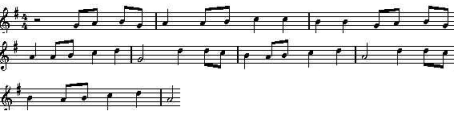
\includegraphics{bildoj/partition.png}
\end{figure}
\begin{verbatim}
por tabako
# Metu en memoron la partituron
sekvenco [0.5 sol la si sol 1 la 0.5 la si 1 :+ do do :- si si 0.5 sol la si sol
          1 la 0.5 la si 1 :+ do re 2 :- sol ]
sekvenco [:+ 1 re 0.5 re do 1 :- si 0.5 la si 1 :+ do re 2 :- la ]
sekvenco [:+ 1 re 0.5 re do 1 :- si 0.5 la si 1 :+ do re 2 :- la ]
sekvenco [0.5 sol la si sol 1 la 0.5 la si 1 :+ do do :- si si 0.5 sol la si sol
          1 la 0.5 la si 1 :+ do re 2 :- sol ]
fino
\end{verbatim}

Por ruli la muzikon, nur restas tajpi: \texttt{tabak muziku}.

Jen nun interesa aplikado de la primitivo \texttt{sekvindp}.  Tajpu la
komandojn:

\begin{verbatim}
sekvv       # Forviŝu la sinsekvon nun en memoro
tabako      # Reŝargu la antaŭan muzikon 
sekvindp 2  # Remetu la kursoron je la nivelo de la unua nigra "la" de la dua mezuro
tabako      # Reŝargu la saman sinsekvon sed prokrastita je du taktoj
muziku      # Grandioza kanono!
\end{verbatim}

Vi povas anka^u ^san^gi l' instrumenton, jen per la komando
\texttt{instrp}, jen en la menu' Agordaj iloj -- Preferoj -- Langeto
Sono.  Vi trovos la liston de ^ciu havebla instrumento kun ^gia numero
(eble en la angla, sed tio ebligas idei; ^ce mi, 411 haveblaj
instrumentoj!).

\section{Bukloj}

XLOGO havas kvin primitivojn ebligantajn efektivigi buklojn:
\texttt{ripetu}, \texttt{ripetupor} kaj \texttt{dum},
\texttt{por\_^ciu}, \texttt{^ciam\_ripetu}.

\subsection{Buklo kun \texttt{ripetu}}

\prim{ripetu}{n listo\_de\_instrukcioj}

$n$ estas entjero kaj \texttt{listo\_de\_instrukcioj} estas listo
enhavanta instrukciojn rulotajn.  L' interpretilo LOGO efektivigos je
$n$ fojoj la komandojn enhavatajn en la listo: tio ^sparas reskribi
$n$ fojojn la saman instrukcioj!  

Ekz:
\begin{verbatim}
ripetu   4 [antaŭen 100 maldekstren 90]    # Kvadrato kun latero 100
ripetu   6 [antaŭen 100 maldekstren 60]    # Seslatero kun latero 100
ripetu 360 [antaŭen   2 maldekstren  1]    # Ee... 360-latero kun latero 2
                                           # Resume, preskaŭ cirklo!
\end{verbatim}
\noindent 
\prim{nombrilon}{}

En buklo \texttt{repete}, estas difinita interna variablo
\texttt{nombrilon}.  Tiu enhavas la numero de l' iteracio kuranta (la
unua iteracio havas numeron $1$).
\begin{verbatim}
ripetu 3 [s nombrilon]
1
2
3
\end{verbatim}

\subsection{Buklo kun \texttt{ripetupor}}

\texttt{ripetupor} ludas la rolon de la bukloj \texttt{for} en aliaj
programlingvoj.

\prim{ripetupor}{listo1 listo2}

Tiu buklo konsistas el doni al variablon kelkajn valorojn en iu
intervalo la^u iu kreskokvanto.

\textit{listo1} enhavas tri parametrojn: la nomon de la variablo, la
komencan limon, la finan limon. Oni povas aldoni kvaran argumenton
nenepran indikantan la kreskokvanton (la pa^son la^u kiu la variablo
mar^sas); se ^gi forestas, apriore valoras $1$.  Jen kelkaj uzadaj
ekzemploj:

\begin{verbatim}
ripetupor [i 1 4] [s :i*2]
2
4
6
8

# Nun oni variigas i inter 7 kaj 2 malkreskante je 1.5 je ĉiu fojo
# Rimarku la negativan kreskokvanton
# Oni skribas post i ĝian kvadraton

ripetupor [i 7 2 -1.5] [s listo :i potencon :i 2] 
7 49
5.5 30.25
4 16
2.5 6.25
\end{verbatim}

\subsection{Buklo kun \texttt{dum}}

\prim{dum}{listo\_testota listo\_de\_instrukcioj}

\textit{listo\_testota} estas listo enhavanta instrukciojn redonantajn bulean.

\textit{listo\_de\_instrukcioj} estas listo enhavanta rulotajn
instrukciojn.  L' interpretilo LOGO rulos refoje
\textit{listo\_do\_instrukcioj} dum \textit{listo\_testota} redonos
``vera''.

Ekz:

\begin{verbatim}
dum ["vera] [dn 1]                    # Testudo turnu sin

# Ekzemplo por skribi renversitan alfabeton

provizu "listo "abcĉdefgĝhĥijĵklmnoprsŝtuŭvz
dum [ne malplena? :listo] [s lastan :listo provizu "listo senlastan :listo]
\end{verbatim}

\subsection{Buklo kun \texttt{por\_^ciu}}

\prim{por\_^ciu}{nomon\_variablan listo\_a^u\_vorto komando}

Tiu primitivo ebligas priskribi ^ciun eron el listo a^u ^ciun signon
el vorto, poste rulas je ^ciu fojo la enhavon de la komandolisto.

\begin{verbatim}
por_ĉiu "i "XLOGO [skribu :i]
X
L
O
G
O
por_ĉiu "i [a b c] [skribu :i]
a
b
c
\end{verbatim}

\subsection{Buklo kun \texttt{^ciam\_ripetu}}

\prim{^ciam\_ripetu}{instrukcilisto}

Ripetu sen fino instrukciliston.

\begin{verbatim}
ĉiam_ripetu [an 1 dn 1]
\end{verbatim}

\textbf{Atentu: uzu tiun primitivon prudente pro la senfina buklo!}

\section{Interkapti la uzulajn agojn}

XLOGO povas interagi kun la uzulo dum la rulado de programo, per
klavaro kaj muso.

\subsection{Interago kun la klavaro}

Oni povas do ricevi tekston de l' uzulo dum ruli la programon, per $3$
primitivoj: \texttt{klave?}, \texttt{litleg} kaj \texttt{leg}.

\prim{klave?}{}

Donu ``vera'' a^u ``malvera'' la^u ^cu oni premis klavon a^u ne post
la komenco de ruli la programon.

\prim{litleg}{}

\begin{itemize}
\item Se \texttt{klave?} estas malvera, haltigu la programon ^gis l'
  uzulo premos klavon.
\item Se \texttt{klave?} estas vera, donu la valoron koncernan al la klavo
  laste premita.
\end{itemize}

\begin{table}[h]
\begin{tabular}{|lllll|}
\hline
A $\Longrightarrow$ $65$ & B $\Longrightarrow$ $66$ & C $\Longrightarrow$ $67$ & ktp... & Z $\Longrightarrow$ $90$\\
\parbox{3cm}{\flushleft $\leftarrow$ $\Longrightarrow$ $-37$ a^u $-226$ (NumKla)} & 
\parbox{3cm}{\flushleft $\uparrow$ $\Longrightarrow$ $-38$ a^u $-224$} &
\parbox{3cm}{\flushleft $\rightarrow$ $\Longrightarrow$ $-39$ a^u $-227$}  & 
\parbox{3cm}{\flushleft $\downarrow$ $\Longrightarrow$ $-40$ a^u $-225$} &\\
Esk $\Longrightarrow$ $27$ & F1 $\Longrightarrow$ $-112$ & F2 $\Longrightarrow$ $-113$ & ... & F12 $\Longrightarrow$ $-123$\\
Uskl $\Longrightarrow$ $-16$ & Spaco $\Longrightarrow$ $32$ & Stir $\Longrightarrow$ $-17$ & Enig $\Longrightarrow$ $10$ &\\
\hline
\end{tabular}
\caption{Kelkaj valoroj de klavoj}
\end{table}

Se vi havas dubon pri la vorto redonata de klavo, sufi^cas tajpi:
\texttt{s litleg}.  L' interpretilo tiam atendos ke vi premos klavon,
poste donos la rilatan valoron.

\prim{leg, legu}{listo1 vor2} 

Afiŝu dialogfenestron kies titro estu \textit{listo1}.  L' uzulo povas
tiam enigi respondon en tekstokampo; la respondon oni konservos kiel
vorton a^u liston (se l' uzulo tajpos plurajn vortojn) en la variablon
\textit{vor2} kiam ^sli validigos a^u klakos la butonon Akceptu.

\subsection{Kelkaj ekzemploj uzi}

\begin{verbatim}
pour juna
 leg [Kiom vi aĝas?] "aĝo
 provizu "aĝo :aĝo
 se :aĝo<18 [s [Vi estas malplenkreskulo]]
 se aŭ :aĝo=18 :age>18 [s [Vi estas plenkreskulo]]
 se :aĝo>99 [s [Mi respektu!!]]
fino

por ralio
    se klave? 
        [provizu "sig litleg
         si :sig=-37 [mdn 90]
         si :sig=-39 [dn  90]
         si :sig=-38 [an  10]
         si :sig=-40 [man 10]
         si :sig=27  [haltu]]
    ralio
fino
# Kontrolu la testudon per la klavaro, haltigu per Esk
\end{verbatim}

\subsection{Interkapti iujn musajn eventojn}

Por tio, oni havas tri primitivojn: \texttt{musleg}, \texttt{muse?}
kaj \texttt{mussit}.

\prim{musleg, muson\_legu}{}

Haltigu la programon ^gis musa evento okazas.  Estas museventoj: movi
la muson a^u klaki iun butonon ^gian.  Okazinte l' evento,
\texttt{musleg} donas nombron ebligantan karakterizi l' eventon.  Jen
la diversaj kodoj asociitaj al la diversaj eventoj:
\begin{itemize}
 \item 0 $\to$ oni movis la muson.
 \item 1 $\to$ oni klakis la butonon $1$ de la muso.
 \item 2 $\to$ oni klakis la butonon $2$ de la muso.
\end{itemize}
La butonoj estas numeritaj de maldekstre al dekstre (principe...).

\prim{mussit, mussituon}{}

Donu liston enhavantan la koordinatojn de la muso dum la lasta interkaptita evento.

\prim{muse?}{}

Donu ``vera'' a^u ``malvera'' la^u ^cu oni agis a^u ne per la muso
post la komenco ruli la programon.

\subsection{Kelkaj uzekzemploj}

En tiu unua proceduro, la testudo sekvas la muson kiam ĝi moviĝas sur la desegnejo.
\begin{verbatim}
por ekzemplo1
# Se oni movas la muson, loku sin al la novan situon
se musleg=0 [sitp mussit]
ekzemplo1
fino
\end{verbatim}

En tiu dua proceduro, estas la sama principo krom ke necesas klaki la
maldekstran butonon musan por movi la testudon sur la desegnejo.
\begin{verbatim}
por ekzemplo2
se musleg=1 [sitp mussit]
ekzemplo2
fino
\end{verbatim}

En tiu tria ekzemplo, ni kreos du butonojn.  Tiu maldekstra ebligos
grafiki kvadraton je $40$ mul $40$ al la dekstro; tiu dekstra,
malgrandan cirklon al la maldekstro.  Finfine, se oni klakos la trian
butonon de la muso, la programo haltos.

\begin{verbatim}
por butono
# kreu ortangulan butonon je 50 mul 100 farbita je salmakoloro
ripetu 2 [an 50 dn 90 an 100 dn 90] 
dn 45 l an 10 ml skolp [255 153 153]
plenigu mal 10 mdn 45 ml skolp 0
fino

por lanĉu
ev butono l skolp [150 0] ml butono
l skolp [ 30   20] ml etikedu "Kvadrato
l skolp [180   20] ml etikedu "Cirklo
l skolp [  0 -100] ml
muso
fino

por muso
# Konservu la rezulton de musleg en la variablon ev
provizu "ev musleg
# Konservu la unuan koordinaton de la muso en la variablon x
provizu "x eron 1 mussit
# Konservu la duan koordinaton de la muso en la variablon y
provizu "y eron 2 mussit
# Se oni klakus la maldekstran butonon
se :ev=1 & :x>0 & :x<100 & :y>0 & :y<50 [kvadrato]
# Se oni klakus la dekstran butonon 
se :x>150 & :x<250 & :y>0 & :y<50 
         [si :ev=1 [cirklo]
          si :ev=3 [haltu]]
muso
fino

por cirklo
ripetu 90 [an 1 mdn 4] mdn 90 l  an 40 dn 90 ml
fino

por kvadrato
ripetu 4 [an 40 dn 90] dn 90 an 40 mdn 90
fino
\end{verbatim} 

\includegraphics*[width=15 cm]{bildoj/lissouris.png}

\subsection{Uzi grafikajn konsista^jojn}

\xlogo{} ebligas anka^u aldoni kelkajn grafikajn konsistaĵojn
(butonon, malvolveblan menuon...) al la desegnejo.  ^Car tiaj
konsista^joj rilatas al grafikaj uzulaj interfacoj, ^ciu primitivo por
tiu afero komenci^gas per la prefikso \og\textsc{gui}\fg.

\subsubsection{Krei konsista^jon}

Por manipuli tiajn grafikajn objektojn, anta^u ^cio necesas krei ilin,
aldoni al ili iujn atributojn, kaj poste afi^si ilin.

\begin{itemize}
\item Por krei butonon:

\prim{gui\_butonon}{vor1 vor2}

Tiu komando kreas butonon kies identiga nomo estas \textit{vor1} kaj
sur kiu estas skribita \textit{mot2}.

Ekzemplo: \texttt{gui\_butonon "b "Klaki}

\item Por krei malvolveblan menuon: 

\prim{gui\_menuon}{vor1 listo2}

Tiu komando kreas menuon kies nomo estas \textit{vor1} enhavantan l'
erojn de la listo \textit{listo2}

Ekzemplo: \texttt{gui\_menuon "m [ero1 ero2 ero3]}
\end{itemize}

\subsubsection{Atribui atributojn al konsista^jo}

\prim{gui\_koordinatojn}{vor1 listo2}

Ebligas loki la grafikan elementon sur la deziratan situon en la
desegnejo.  Ekzemple, por loki la anta^uan butonon al punkto kun
koordinatoj $(20;100)$, skribu:

\begin{verbatim}
 gui_koordinatojn "b [20 100]
\end{verbatim}

Se la situo de la konsista^jo ne estas indikita, la konsista^jo estos
lokita apriore je la supra maldekstra angulo de la desegnejo.

\prim{gui\_forigu}{vor1}

Forvi^su grafikan elementon.  Ekzemple, por forigi la anta^uan
butonon:
\begin{verbatim}
 gui_forigu "b
\end{verbatim}

\prim{gui\_agadon}{vor1 listo2}

Difinu agadon realigendan kiam l' uzulo interagos kun la grafika
elemento konsiderita.

\begin{verbatim}
# La testudo anta^uen iru 100 paŝojn se oni klakos butonon "b
gui_agadon "b [an 100]

# Por la malvolvebla menuo, ^ciu ero havas sian propran agon
gui_agadon "m [[skrbiu "ero1]  [skribu "ero2] [skribu "ero3]]
\end{verbatim}

\prim{gui\_desegnu}{vor1}

Afi^su la grafikan konsista^jn sur la desegnejon.  Ekzemple, por montri la butonon:
\begin{verbatim}
 gui_desegnu "b
\end{verbatim}

\section{Administri la tempon}

\xlogo{} havas plurajn primitivojn ebligantajn koni la horon, la daton
a^u anka^u administri nombradojn (utilaj por ripetu taskon la^u
fiksitaj intervaloj).

\prim{atnd, atendu}{n}

Haltu la programon kaj do la testudon dum $n$ 60\textsuperscript{onoj}
de sekundo.

\prim{tmpko, tempokomencon}{n}

Komencu nombri $n$ sekundojn.  Oni povas scii ^cu la nombrado estas
finita per la primitivo \texttt{tmpfi}.

\prim{tmpfi, tempofine?}{}

Donu \texttt{"vera} se neniu nombrado estas aktiva.  Donu
\texttt{"malvera} se la nambrado ne estas finita.

\prim{daton}{}

Redonu liston konsistantan el tri entjeroj prezentantaj la daton.  La
unuo indikas la tagon.  La dua la monaton.  La tria la jaron.
$\Longrightarrow$ [tago monato jaro]

\prim{horon}{}

Donu liston kun tri entjeroj prozentantaj la horon.  La unua prezentas
la horojn, la dua la minutojn kaj la lasta la
sekundojn. $\Longrightarrow$ [horo minuto sekundo]

\prim{tmp, tempon}{}

Donu la tempon pasintan de post la starto de \xlogo.  Tiu tempo estas
esprimata en sekundoj.

Jen malgranda proceduro ekzemplo:
\begin{verbatim}
por horloĝo
# afiŝu la horon en formo cifera
# (ĝisdatigu l' afiŝadon je ĉiu 5 sekundoj)
se tmpfi 
  [ev 
   tiparon\_provizu 75 
   tdk
   provizu "hor horon
   provizu "h unuan :hor
   provizu "m er 2 :hor
   # afiŝi je du ciferoj la minutojn (oni aldonas la 0)
   se :m-10 < 0 [p "m vort 0 :m]
   p "s lastan :hor
   # afiŝi je du ciferoj la sekundojn
   se :s-10 < 0 [p "s vort 0 :s]
   etikedu vort vort vort vort :h ": :m ": :s 
   tmpko 5]
horloĝo
fino
\end{verbatim} 

\section{Uzi la reton kun XLogo}
\label{reseau}

\subsection{La reto: kiel ^gi funkcias?}

Anta^u ^cio, en ^ci tiu enkonduko, necesas klarigi kelkajn konceptojn
por bone kompreni la uzadon de la primitivoj.

\begin{figure}[h]
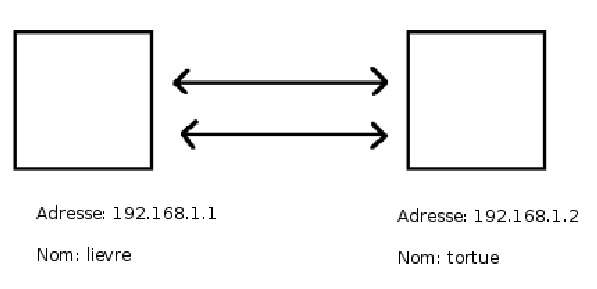
\includegraphics{bildoj/reseau.png}
\caption{Nocio de reto}
\end{figure}

Du komputiloj povas komuniki tra la reto se ili havas retkarton
(ethernet) a^u similan rimedon.  Al ^ciu komputilo oni donas personan
adreson: \textit{^gia adreso~IP}.  Tiu adreso IP konsistas el $4$
entjeroj inter $0$ kaj $255$, disigitaj de punktoj.  Ekzemple, l'
adreso IP de la unua komputilo en la anta^ua skemo estas 192.168.1.1.

^Car ne facilas memori tiajn adresojn, eblas ankaŭ rilatigi al ^ciu
adreso IP nomon pli kutiman pli facile memoreblan.  Sur la anta^ua
skemo, oni povas adresi sin al la dekstra komputilo jen vokante ^gin
per ^gia IP-adreso 192.168.1.2, jen vokante ^gin per ^gia nomo
\texttt{tortue}.

Mi ne parolos pli pri la signifojn de tiuj nombroj.  Mi aldonos nur
ion bonan por scii: la loka komputilo sur kiu oni laboras havas ^ciam
specifan IP-adreson, 127.0.0.1 (krom eble alia a^u aliaj IP-adresojn);
^gi havas specifan nomon, ofte \texttt{localhost} (krom eble alia a^u
aliaj nomoj).

\subsection{Porretaj primitivoj} 

XLogo havas $4$ primitivojn ebligantajn komuniki per reto:
\texttt{tcp\_a^uskultu}, \texttt{ekzekucutcp}, \texttt{diskutilotcp}
kaj \texttt{sendutcp}.  Por la sekvaj ekzemploj konsideru ^ciam la
okazo de la du komputiloj de la anta^ua skemo.

\prim{tcp\_a^uskultu, tcp\_auskultu, tcp\_awskultu, tcp\_auxskultu}{}

^Gi estas la bazo de ^ciu retkomunikado.  ^Gi ekspektas neniun
argumenton.  ^Gi ebligas ke komputilo rulanta ^gin a^uskultu ordonojn
donitajn de aliaj komputiloj en la sama reto.

\prim{ekzekucutcp}{vor1 listo2}

Tiu primitivo ebligas ruli instrukciojn sur iu komputilo en la reto.

\textit{vor1} indikas la IP-adreson a^u la nomon de la vokata komputilo,
\textit{listo2} enhavas la rulotajn instrukciojn.

Ekzemple: Mi estas sur la komputilo \texttt{lievre}, mi deziras
grafiki kvadraton kun latero $100$ sur l' alia komputilo.  Tial,
necesas ke sur la komputilo \texttt{tortue} mi rulu la ordonon
\texttt{tcp\_a^uskultu}; poste, sur la komputilo \texttt{lievre}, mi
rulu:
\begin{verbatim}
ekzekucutcp "192.168.1.2 [ripetu 4 [an 100 dn 90]]
\end{verbatim}
ou 
\begin{verbatim}
exekucutcp "tortue [ripetu 4 [an 100 dn 90]]
\end{verbatim}

\prim{diskutilotcp}{vor1 listo2}

^Gi ebligas dialogi inter du komputiloj de la reto, afi^sante
fenestron ebligantan la interparolon.

\textit{vor1} indikas la IP-adreson a^u la nomon de la vokita
komputilo, \textit{listo2} enhavas la frazon afi^sotan.

Ekzemple: \texttt{lievre} volas diskuti kun \texttt{tortue}.

\texttt{tortue} rulu \texttt{tcp\_a^uskultu} por meti sin en atendon
de peto far komputiloj en la reto.  \texttt{lievre} rulu tiam:
\texttt{diskutilotcp~"192.168.1.2~[saluton]}.

Du fenestroj ebligantajn la dialogon malfermi^gas tiam sur ^ciu
komputilo.

\prim{sendutcp}{vor1 listo2} 

Sendu datumojn al komputilo de la reto, poste donu la respondon de la
alia komputilo.

\textit{vor1} indikas la IP-adreson a^u la nomon de la komputilo
vokata, \textit{listo2} enhavas la datumojn sendotajn.  Se la
komunikado fari^gos kun alia komputilo kie \xlogo{} ruli^gas, tiu
komputilo respondos OK post fini l' operacion.  Eblas anka^u dialogi
kun roboto havanta retan interfacon, sed la respondo povos esti
malsama tiam.

Ekzemple: 

\texttt{tortue} volas sendi al \texttt{lievre} la sinsekvon ``3.14159
preska^u la nombro pi''.

\texttt{lievre} rulu \texttt{tcp\_a^uskultu} por atendi peton far
komputiloj de la reto.  \texttt{tortue} rulu tiam:
\texttt{skribu~sendutcp~"lievre~[3.14159 preska^u la nombro pi]}.

\textbf{Jen konsileto:} Ekrulu du fojojn XLogo sur la sama komputilo.
\begin{itemize}
 \item En la unua fenestro, rulu \texttt{tcp\_a^uskultu}.
 \item En la dua, rulu \texttt{ekzekucutcp "127.0.0.1 [an 100 dn 90]}
\end{itemize}

Vi tiel movis la testudon sur l' alian fenestron!
